\documentclass[11pt]{article}

\usepackage{latexsym}
\usepackage{amsmath}
\usepackage{amssymb}
\usepackage{amsthm}
\usepackage{graphicx}
\usepackage{wrapfig}
\usepackage{pseudocode}
\usepackage{url}
\usepackage[backref, colorlinks=true, citecolor=red, urlcolor=blue, pdfauthor={Jyh-Ming Lien}]{hyperref}
\usepackage{subfig}


\newcommand{\handout}[5]{
  \noindent
  \begin{center}
  \framebox{
    \vbox{
      \hbox to 5.78in { {\bf } \hfill #2 }
      \vspace{4mm}
      \hbox to 5.78in { {\Large \hfill #5  \hfill} }
      \vspace{2mm}
      \hbox to 5.78in { {\em #3 \hfill #4} }
    }
  }
  \end{center}
  \vspace*{4mm}
}

\newcommand{\lecture}[4]{\handout{#1}{#2}{#3}{#4}{#1}}

\newtheorem{theorem}{Theorem}
\newtheorem{corollary}[theorem]{Corollary}
\newtheorem{lemma}[theorem]{Lemma}
\newtheorem{observation}[theorem]{Observation}
\newtheorem{proposition}[theorem]{Proposition}
\newtheorem{definition}[theorem]{Definition}
\newtheorem{claim}[theorem]{Claim}
\newtheorem{fact}[theorem]{Fact}
\newtheorem{assumption}[theorem]{Assumption}

% 1-inch margins, from fullpage.sty by H.Partl, Version 2, Dec. 15, 1988.
\topmargin 0pt
\advance \topmargin by -\headheight
\advance \topmargin by -\headsep
\textheight 8.9in
\oddsidemargin 0pt
\evensidemargin \oddsidemargin
\marginparwidth 0.5in
\textwidth 6.5in

\parindent 0in
\parskip 1.5ex
%\renewcommand{\baselinestretch}{1.25}

\begin{document}

\lecture{Two algorithms for two-dimensional bin packing problems}{Genqian Hu}{CS 633 Computational Geometry}

\begin{abstract}
The final project is to implement 2 algorithms for 2-dimensional bin packing problem from a paper. The one algorithm of the 2 algorithm is for 2BPRG and the other one is for 2BPRF. And both of them use a value correction procedure to update the value of each item after the generation of cutting plans.
\end{abstract}

\section{Motivation and Introduction}
Code: git clone https://github.com/tex775306106/CS633FinalProjectBinPacking
\vspace{3mm}
\newline
Packing problem is one of the classical problems in Computational Geography. In that problem, many items with different shapes are packed into many containers usually with the same size. The object of it is to minimize the total number of containers needed to pack all the items. For an instance, it's like a express company wants to minimize the number of the trucks but delivers the same number of packages. In bin packing problem, containers are all cuboid bins. Bin packing problem is a combinatorial NP-hard problem. And it's NP-complete to decide whether the given bins are enough to pack all items.
\newline
The 2-dimensional bin packing problem is one variation of the packing problem. If all the items are triangles, then there are 4 cases for this problem.
\newline
1.	2BPOG: Items' orientation is fixed, and guillotine cuts are required.
\newline
2.	2BPRG: Items can be rotated by 90 degrees, and guillotine cuts are required.
\newline
3.	2BPOF: Items' orientation is fixed, and guillotine cuts are not required.
\newline
4.	2BPRF: Items can be rotated by 90 degrees, and guillotine cuts are not required.
\newline
A paper introduces two sequential heuristic algorithms to solve the 2BPRG and 2BPOF problems. Both algorithms are based on a value correction algorithm that after each cutting plan generation, each item's value is updated. The object is to maximize the total value of each bin.

\section{Methods Used and Studied}
    \subsection{Algorithm for 2BPRG}

        \subsubsection{Strip}
        A strip can contain many items. And the items are placed along the same edge of the strip one by one. The width of the strip is one of the length of width of the items inside the strip. The length of the strip is the sum of the length of the edges of the items along the same edge of strip. For a given length, if there are m remaining items, 2m kind of strips should be considered as each edge of an item can be the width of a strip. Figure 1 is a strip with 4 items inside.
        \newline
	    In this algorithm, after each guillotine cut, exactly one strip will be cut out except the last move generates two strips.
        \begin{figure*}
        \begin{minipage}[hb]{0.5\linewidth}
        \centering
        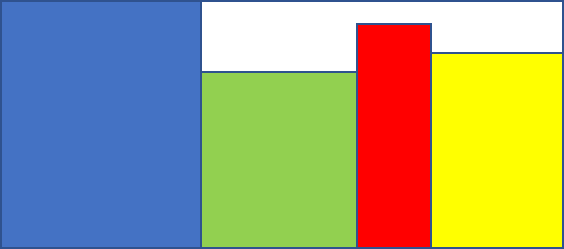
\includegraphics[width=0.8\textwidth]{FIGS/examples/1.png}
        \caption{a strip}
        \label{skyline}
        \end{minipage}

        \end{figure*}
        \subsubsection{Strip packing order}
        Instead of packing items, this algorithm puts strip into the bin as the combination of items. For a sub-bin with size x*y, there are 2 ways of packing a strip. If the width of the strip is W, then 2 kinds of strips needs to be compared. The first way is to put a strip with size W*x along the upper edge of the bin. Or the other way is to pack a strip with size W*y along the right edge of the bin. The algorithm uses a recursion to determine which move gets higher value.
        \newline
        If packing the strip horizontally along the upper edge is better, the effective value of the strip is calculated. For every item inside the strip, if it has not been put into any bins, it contributes to the effective value of this strip. If the strip has no effective value to the current pattern, the stirp will be skipped. Or the strip is packed and the effective value of each item in other strips should be updated as they may include packed items. The process of acing a strip along the right edge is similar.
    \subsection{Algorithm for 2BPRF}
    For this algorithm, items are sorted in non-increasing order to improve the performance.
        \subsubsection{Candidate Position}
        For each bin, the first item is placed at the left bottom corner. Then all the following items must be placed at a candidate position. And boundary of the available area is from top left corner to right bottom corner which should be a downward stair shape. A candidate position refers to where the boundary turns form a vertical edge to a horizontal edge at a inflection point. In figure 2, the top left point, the right bottom point of the yellow triangle and the right bottom point of the blue triangle are the all three candidate points.
        \subsubsection{Available Space}
        In figure 3, a red triangle is placed at the last candidate point, which makes the boundary oscillate. To let the boundary keep a non- increasing trend, the hill shape free space is marked as unavailable space and abandoned. Thus, the two candidate positions in figure 4 are the top left point of the black polygon and the right bottom point of the red triangle.
        \newline
        In the original paper, if a part of the space is too to fit any remaining item, that part of space will be marked as bad region which is also the unavailable space. But the computation cost is too much to check every part of the available space for all remaining items when an item is packed. Instead, I just check whether a candidate position is feasible when considering putting an item into the bin.
        \begin{figure*}
        \begin{minipage}[hb]{0.33\linewidth}
        \centering
        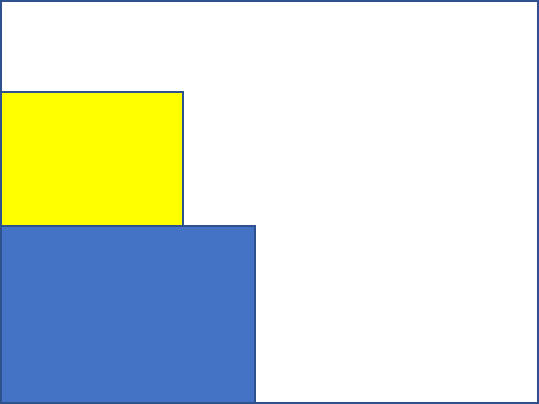
\includegraphics[width=0.8\textwidth]{FIGS/examples/2.png}
        \caption{2 items packed}
        \label{skyline}
        \end{minipage}
        \begin{minipage}[hb]{0.33\linewidth}
        \centering
        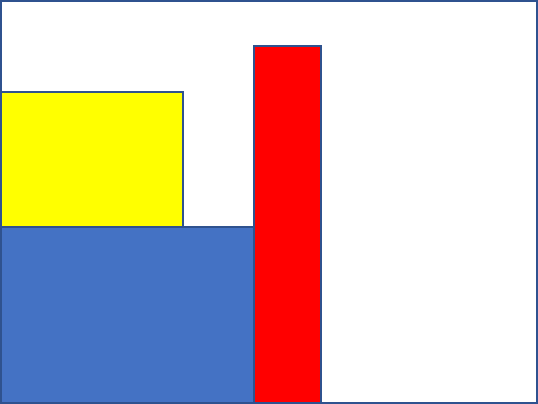
\includegraphics[width=0.8\textwidth]{FIGS/examples/3.png}
        \caption{3 items packed}
        \label{skyline}
        \end{minipage}
        \begin{minipage}[hb]{0.33\linewidth}
        \centering
        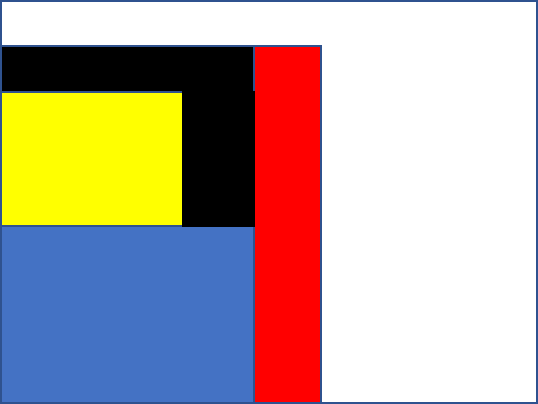
\includegraphics[width=0.8\textwidth]{FIGS/examples/4.png}
        \caption{equivalent area }
        \label{skyline}
        \end{minipage}
        \end{figure*}
        \subsubsection{Items Packing Order}
        The packing order of the items is based on greedy procedure. Most of the running time are consumed at this part, because it checks all items for all candidate points to pre-compute which item leads to the largest value of the bin if it's placed there.
        \newline
        When considering packing an item at a specific candidate position, the algorithm calculates its lower bound first. And the lower bound of the item for a candidate position is that it assumes the item is placed at that candidate position, then it keeps putting remaining items into the bin until the bin is full or all items are packed. But when packing remaining items, all candidate positions are checked for each remaining item. And the boundary of the available space is updated each time an item is packed. After all this, the total value of the bin is the lower bound for packing that item at the candidate position. The pattern of the bin is discard.
        \newline
        For each candidate position, all remaining items' lower bounds need to be computed to know what is the best move for packing a single item into the bin. After that, the available space is updated and the lower bounds for the new boundary are computed.
        \newline
        For all candidate position, when the lower bounds for all remaining items are all 0, it means the remaining available space of the bin is too small or all items are packed into bins.
        \subsubsection{EA and GN}
        After putting an item into the bin, if a space larger than the size of the item itself is unavailable space like the red triangle and black polygon in figure 4. Then, the size of the black polygon and red triangle together is the equivalent area(EA) to the red triangle.
        \newline
        When computing the lower bound, the item with smaller equivalent area is better. I use the difference of areas of the space below the boundary before and after an item is packed as the equivalent area.
        \newline
        If multiple items have the equivalent area, the goodness value(GN) of each of them are computed. For each item, when the length of the triangle exactly matches the length of the edge of the boundary below it or the height of the triangle is the same as the length of the edge of the boundary left to it, GN is 1. If both edges match, GN is 2. The item with higher GN is considered as the better choice here.
    \subsection{Value Correction}
    According to the authors, it is the highlight of the original paper. After each cutting plan, the value of each item is updated so that items which don't fit the current plan well will be packed sooner. The value correction of its each item is related to its value in the former cutting plan and the utility of bins. So, it's like a gradient decent algorithm.
\section{Results}
    \subsection{Implementation Discuss}
    I implement the algorithms in C++ with Visual Studio 2015. And OpenCV3.1(x64) is used to output patterns of bins.
        \subsubsection{Algorithm for 2BPRG}
        I implement this algorithm in a different way from what the paper introduces, but the idea is the same. In the original paper, the x and y start from 0 to expand the sub-bin. And I let x be the length of the bin and let y be the height of the bin to shrink the sub-bin.
        \newline
        Although I believe each implemented function of the algorithm works correctly, I am still debugging the codes to let it perform better on larger size of bins or more items. For now, it can only work on several items and small size of bins. Otherwise, the F(x,y) recursion function may consume hours. I think the reason is that I the conditional statement I set to end the loop is not efficient for some cases or some parts of the code are repetitive.
        \subsubsection{Algorithm for 2BPRF}
        When implementing this algorithm, the most challenge part is updating the boundary of available space correctly. Because there are more than 10 cases of placing an item to a candidate position. To avoid of neglecting special cases, I classify each case into one of the four cases (no item packed, pack to the first candidate position, pack to the last position, pack to a general candidate point). And when a item is placed, the length and height of it can be longer, shorter or the same as the adjacent edge of the boundary. So there are at least 9 cases for considering all pairs of them.

    \subsection{Results}
    \begin{figure*}
    \begin{minipage}[htb]{0.33\linewidth}
    \centering
    \includegraphics[width=0.8\textwidth]{FIGS/1/output1.png}
    \caption{bin 1 before value correction}
    \label{skyline}
    \end{minipage}
    \begin{minipage}[htb]{0.33\linewidth}
    \centering
    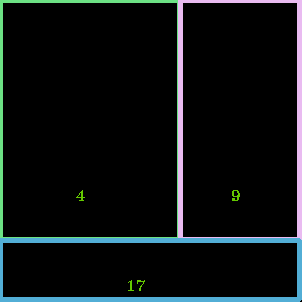
\includegraphics[width=0.8\textwidth]{FIGS/1/output2.png}
    \caption{bin 2 before value correction}
    \label{skyline}
    \end{minipage}
    \begin{minipage}[htb]{0.33\linewidth}
    \centering
    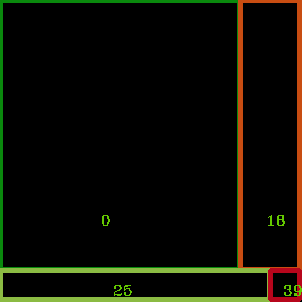
\includegraphics[width=0.8\textwidth]{FIGS/1/output3.png}
    \caption{bin 3 before value correction}
    \label{skyline}
    \end{minipage}
    \end{figure*}
    \begin{figure*}
    \begin{minipage}[htb]{0.33\linewidth}
    \centering
    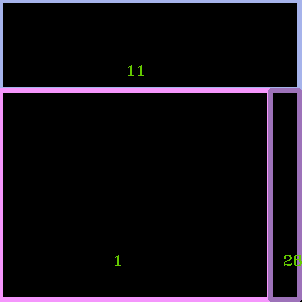
\includegraphics[width=0.8\textwidth]{FIGS/1/output4.png}
    \caption{bin 4 before value correction}
    \label{skyline}
    \end{minipage}
    \begin{minipage}[htb]{0.33\linewidth}
    \centering
    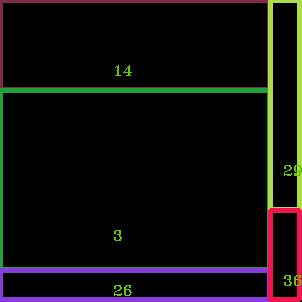
\includegraphics[width=0.8\textwidth]{FIGS/1/output5.png}
    \caption{bin 5 before value correction}
    \label{skyline}
    \end{minipage}
    \begin{minipage}[htb]{0.33\linewidth}
    \centering
    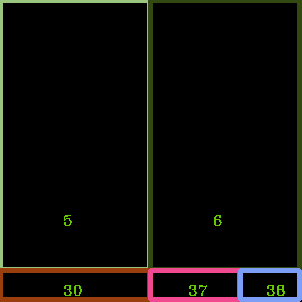
\includegraphics[width=0.8\textwidth]{FIGS/1/output6.png}
    \caption{bin 6 before value correction}
    \label{skyline}
    \end{minipage}
    \end{figure*}
    \begin{figure*}
    \begin{minipage}[htb]{0.33\linewidth}
    \centering
    \includegraphics[width=0.8\textwidth]{FIGS/1/output7.png}
    \caption{bin 7 before value correction}
    \label{skyline}
    \end{minipage}
    \begin{minipage}[htb]{0.33\linewidth}
    \centering
    \includegraphics[width=0.8\textwidth]{FIGS/1/output8.png}
    \caption{bin 8 before value correction}
    \label{skyline}
    \end{minipage}
    \begin{minipage}[htb]{0.33\linewidth}
    \centering
    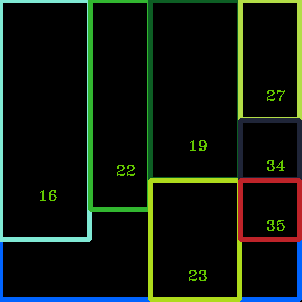
\includegraphics[width=0.8\textwidth]{FIGS/1/output9.png}
    \caption{bin 9 before value correction}
    \label{skyline}
    \end{minipage}
    \begin{minipage}[htb]{0.33\linewidth}
    \centering
    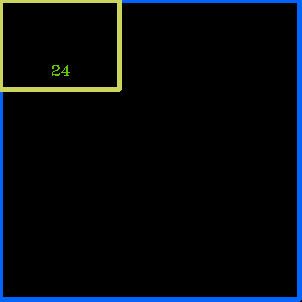
\includegraphics[width=0.8\textwidth]{FIGS/1/output10.png}
    \caption{bin 10 before value correction}
    \label{skyline}
    \end{minipage}
    \end{figure*}

    \begin{figure*}
    \begin{minipage}[htb]{0.33\linewidth}
    \centering
    \includegraphics[width=0.8\textwidth]{FIGS/2/output1.png}
    \caption{bin 1 after value correction}
    \label{skyline}
    \end{minipage}
    \begin{minipage}[htb]{0.33\linewidth}
    \centering
    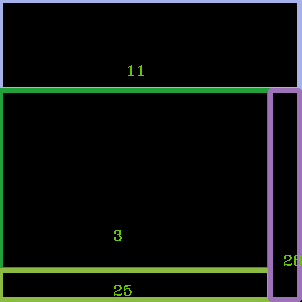
\includegraphics[width=0.8\textwidth]{FIGS/2/output2.png}
    \caption{bin 2 after value correction}
    \label{skyline}
    \end{minipage}
    \begin{minipage}[htb]{0.33\linewidth}
    \centering
    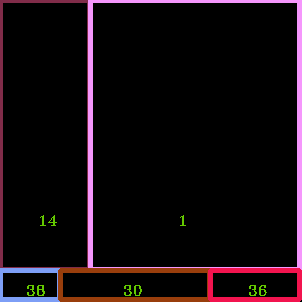
\includegraphics[width=0.8\textwidth]{FIGS/2/output3.png}
    \caption{bin 3 after value correction}
    \label{skyline}
    \end{minipage}
    \end{figure*}
    \begin{figure*}
    \begin{minipage}[htb]{0.33\linewidth}
    \centering
    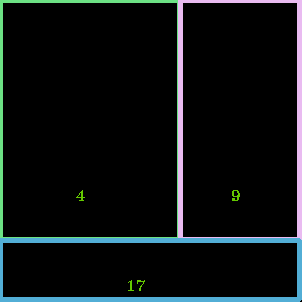
\includegraphics[width=0.8\textwidth]{FIGS/2/output4.png}
    \caption{bin 4 after value correction}
    \label{skyline}
    \end{minipage}
    \begin{minipage}[htb]{0.33\linewidth}
    \centering
    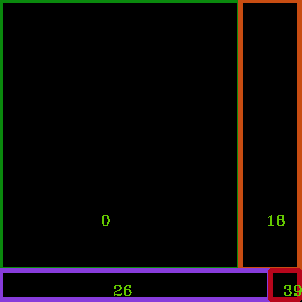
\includegraphics[width=0.8\textwidth]{FIGS/2/output5.png}
    \caption{bin 5 after value correction}
    \label{skyline}
    \end{minipage}
    \begin{minipage}[htb]{0.33\linewidth}
    \centering
    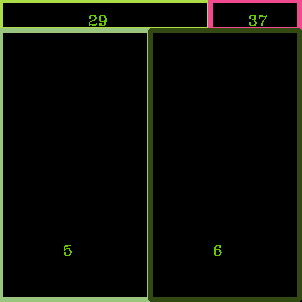
\includegraphics[width=0.8\textwidth]{FIGS/2/output6.png}
    \caption{bin 6 after value correction}
    \label{skyline}
    \end{minipage}
    \end{figure*}
    \begin{figure*}
    \begin{minipage}[htb]{0.33\linewidth}
    \centering
    \includegraphics[width=0.8\textwidth]{FIGS/2/output7.png}
    \caption{bin 7 after value correction}
    \label{skyline}
    \end{minipage}
    \begin{minipage}[htb]{0.33\linewidth}
    \centering
    \includegraphics[width=0.8\textwidth]{FIGS/2/output8.png}
    \caption{bin 8 after value correction}
    \label{skyline}
    \end{minipage}
    \begin{minipage}[htb]{0.33\linewidth}
    \centering
    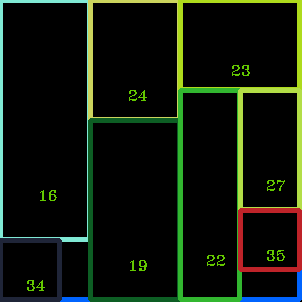
\includegraphics[width=0.8\textwidth]{FIGS/2/output9.png}
    \caption{bin 9 after value correction}
    \label{skyline}
    \end{minipage}

    \end{figure*}

    For the guillotine cuts algorithm, now it works for calculating the number of needed bins for small number of items and little bins. Using larger bins takes much more time in recursions.
    \newline
    The implementation for free cuts cutting plan generation is done. I use the same data which the authors of the paper use for testing algorithm for 2BPRG to test it. Figure 5 to 14 show the result for the first cutting plan. Because OpenCV takes the top left as the origin of the coordinate axis. So the first item is placed at the top left corner of each bin. The triangles with a number are the items with its id. Other polygons are unavailable space. According to the result, these 40 items need 10 bins to pack all them. However, the optimal solution is 9 bins. Figure 15 to 23 are the outputs of the algorithm after a value correction process, which packs all items with 9 bins. According to these outputs, some patterns change after the value correction. It proves the value correction works successfully. But I also find if the algorithm continues running, the solution may go back to 10 bins.

\section{Conclusion}
    Both algorithms are sequential heuristic algorithm and they are involved with many recursions and for loop nests. So when the size of bin is not small or there are more than a few items, it takes really long time to work them out. But the output is not bad for the free cuts, because it demonstrates that the solution it gives is nearly optimal and the value correction works fine. So these algorithms may give other researchers an idea of how to update items' value.
\begin{thebibliography}{5}
\bibitem{ref1}[1]Y.  Cui, Y.  Cui and T.  Tang, "Sequential heuristic for the two-dimensional bin-packing problem", European Journal of Operational Research, vol. 240, no. 1, pp. 43-53, 2015.
\end{thebibliography}

\end{document}


